\section{Dynamic scalability} 
\label{sec:dynamic_scalability} 

In this section, we explain how our system design enables view 
maintenance to dynamically scale in and out. We first describe 
a couple of fundamental management operations that specify how single 
components can be added or removed from the system and how they are 
properly integrated in the view processing. Next, we show that for these 
runtime management operations still all requirements for strong consistency 
(cf. Theorem~\ref{theo:strong_consistency}) are fulfilled, which
eventually guarantees consistency as described in 
Section~\ref{sec:consistency}. 

\subsection{Management procedures} 
\label{sec:management_procedures} 

So far, we were assuming a basic system configuration where a fixed 
number of nodes is statically assigned to a fixed number of view 
managers. Load peaks, however, require the system to process increased 
amounts of updates for certain time spans. Without decently adapting the 
system, the view maintenance process could be either significantly delayed, 
or even crash due to overloaded components. To automatically 
encounter these situations, i.e., scale the view maintenance processing 
and re-balance the load, (1) new components need to be properly added or 
removed during runtime, and (2) existing components must potentially be 
reassigned. We therefore define the following system \textit{management 
operations}: 

\noindent
\textbf{Add view manager -- } This operation handles the addition of a 
new VM to the pool of available system resources. During bootstrap, an 
upcoming VM first contacts a given Zookeeper ensemble and registers 
there. The coordinator, in turn, is notified about the registration and 
updates its own configuration. By default the newly added VM is in state 
\textit{idle}, i.e., it waits until the coordinator assigns it to a 
node. 

\noindent
\textbf{Assign view manager -- }This procedure describes how an 
\textit{idle} VM is assigned to the NX of a particular node. The 
coordinator initiates this procedure by sending an assignment command, 
which contains the address of the target node, to the VM. The remaining 
assignment steps are handled without further involvement of the 
coordinator. First, the VM sends a request to the desired node (i.e. 
NX). The NX, in turn, assigns the VM by (1) adding a reference to its 
hash-ring, (2) creating an outbound queue to buffer all future update 
operations according to the consistent hashing function, and (3) 
starting a separate thread to propagate these update operations. To 
complete the assignment, the NX acknowledges the successful assignment 
to the VM, which forwards the acknowledgment to the coordinator that 
updates is configuration and thereby completes the operation. 

\noindent
\textbf{Withdraw view manager -- } This procedure removes an existing 
assignment of a particular VM from its NX. It is initiated by the 
coordinator that sends a withdraw command to the VM. This command is 
forwarded to the associated NX, which essentially undoes the assignment 
operations. It first removes the reference from the hash-ring, so no 
more updates get assigned to the VM. After all remaining update 
operations in the queue are propagated, the queue-handling thread is 
closed down and an acknowledgement is sent to the VM. This message is 
again forwarded to the coordinator that updates its configuration and 
thereby completes the operation. Note that a successful withdrawal does 
only change the state of the VM back to \textit{idle} but does not 
terminate the process itself. The VM remains in the system's resource 
pool and can be later used again. 

\noindent
\textbf{Remove view manager -- } In contrast to withdrawing, this 
procedure also terminates the VM process and thereby deletes it from the 
system's resource pool. This operation can be either initiated by the 
coordinator --- sending an explicit remove command --- or by the VM 
itself. To enable a controlled removal, the VM first performs a 
\textit{withdraw} procedure, to close the assignment. After receiving 
the respective acknowledgement from the coordinator, the VM process 
terminates. This deletes the session node in the Zookeeper ensemble, 
which informs the coordinator about the eventual disappearance of the 
node. Again, the coordinator updates its configuration and the procedure 
is completed. 

\noindent
\textbf{Reassign view manager -- } A reassignment is used to move an 
already existing and currently assigned view manager from one NX to a 
new NX. The procedure is initiated by the coordinator that sends a 
reassign command to the VM. First, the VM performs a \textit{withdraw} 
procedure to close the old assignment, and then an \textit{assign} 
procedure to register itself at the new NX. Once the VM receives the 
confirmation about the successful assignment from the new NX, an 
acknowledgement is sent to the coordinator that updates its 
configuration. 

\subsection{Consistency review} 
\label{subsec:consistency_review} 

By now, we only analysed the consistency in a static context. A fixed 
number of nodes and view managers has been assumed. Now, that our system 
operates in a dynamic context, consistency has to be reviewed again. The 
following example shows why the newly introduced management functionality 
reveals a potential to violate view consistency if no additional 
countermeasures are taken into consideration. 

\textit{Example 3:} Let $A(\underline{K}, F)$ be the base table for this 
example. Assume a client $c_1$ performing a put operation $t_1(A(k_1, 
\{..\}))$ and let's further assume the NX selects $VM_2$ as the next 
responsible view manager for $k_1$. Then, $t_1$ is put to the queue of $VM_2$. 
Now assume, a view manager $VM_3$ is assigned to the NX and that $VM_3$ 
acquired the responsibility for key $k_1$. It is inserted into the hash-ring 
and a new queue is created. In a next step, client $c_1$ sends an update $t_2 
(A(k_1, \{..\}))$, which is now added to the queue of $VM_3$. Considering, 
that $VM_3$ has just been added, it's queue is comparatively empty and hence 
processing very fast. It is likely to happen that $VM_3$ processes $t_2$ 
before $VM_2$ can process $t_1$. Because both operations refer to the same 
base record, the time-line of the record is changed. As explained before, this 
has to be prevented in order to preserve convergence of views. 

The solution we suggest, is using so called \textit{markers}. Markers identify 
a certain change in NX component (e.g., the addition of a new $VM$ to the hash 
ring) and can be inserted into the queue of view managers. Markers are sent 
just like updates to view managers. When a view manager recognizes a marker, 
it replies with an acknowledgement to the NX indicating that this particular 
$VM$ has seen and processed all updates that have been added to the $VM$'s 
queue before the marker was added. We use this property to solve the time-line 
problem in Example~3. 

To realize the marker mechanism, we adapted parts of the NX and VM 
implementation. At the VM side only minor changes are necessary. If a VM 
receives an update operation it is processed as usual. If it receives a 
marker, an acknowledgement containing a marker id is sent back to the NX. 
However, the logic on the NX side is slightly more subtle and in the following 
we base our description on a set of primitive operations. These include 
methods that are needed by the NX component to assign (or withdraw) VMs to (or 
from) itself: (i) $createQueue(vm)$ creates a new queue for a particular view 
manager and (ii) $deleteQueue(vm)$ removes an existing queue for a particular 
view manager. The queue for a VM can only be deleted, if it is empty and no 
update operation is queued. (iii) $queueOperation(vm, bto)$ inserts, either a 
base table operation, or a marker into the queue of a particular view manager. 
The methods (iv) $activateQueue(vm)$ and (v) $deactivateQueue(vm)$ start or 
stop the sending thread that keeps transferring the operations in the queue 
for a particular VM. A view manager can be added to the hash ring by (vi) 
$insertHash(vm)$, or removed from the hash ring by (vii) $removeHash(vm)$. For 
the communication between components, we use the simple methods (viii) 
$sendMessage()$ and the method (ix) $receiveMessage()$. Now, we are able to 
refine the system's key procedures defined before. 

\noindent
\textbf{Assign view manager -- } When a view manager is assigned, it 
is added to the hash-ring of the NX component. Unless the hash-ring 
is empty, the new view manager is assigned a key region that is, at the same 
time, withdrawn from another view manager. In 
Figure~\ref{fig:review_consistency}, a view maintenance process of a NX 
is shown. Recall, that the NX selects the responsible view manager for the 
updates by applying the consistent hash function. The update is then inserted 
into the corresponding queue. 


\begin{figure}[h!]
  \centering
    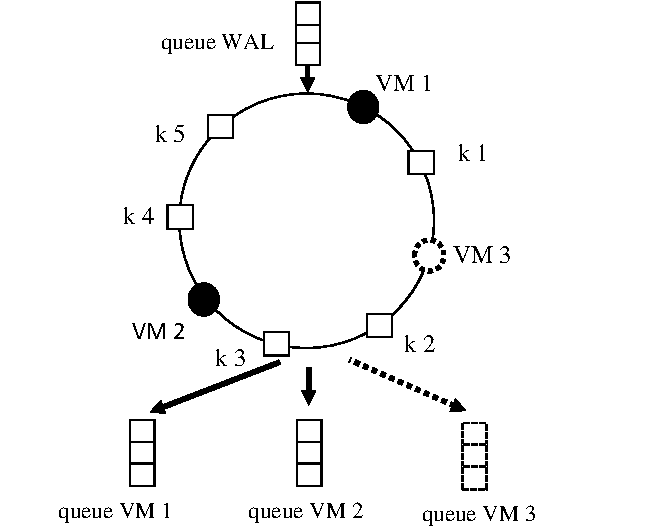
\includegraphics[width=\linewidth]{figures/ReviewConsistency}
        \vspace{-7mm}
    \caption{Review consistency}
        \vspace{-3mm}
    \label{fig:review_consistency}
\end{figure}

We change the assignment procedure by adding the marker-based acknowledgement mechanism (cf. Algorithm~\ref{alg:assignvm}). The algorithm is executed synchronously and if another assignment procedure is called on the NX, it has to wait, until the first operation has terminated.
  
\begin{algorithm}
\caption{Secure assignment procedure at NX}
\label{alg:assignvm}
\begin{algorithmic}[5]
\Procedure{$assignVm$}{$vm_a, VM_{nx}$}
\State $createQueue(vm_a)$\Comment{create queue for VM}
\State $insertHash(vm_a)$\Comment{add VM to hashring}
\ForAll{$vm \in VM_{nx}$}
\State $queueMarker(vm, m_a)$\Comment{queue marker}	
\EndFor
\ForAll{$vm \in VM_{nx}$}\Comment{wait for answers}	
\State $receiveMessage(VM, m_a)$	
\EndFor
\State $activateQueue(vm_a)$\Comment{activate queue}	
\EndProcedure
\end{algorithmic}
\end{algorithm}
  
The procedure $assignVm$ takes two parameters: $vm_a$, the view manager 
that should be assigned to the NX component, and $VM_{nx}$, a set of view 
managers that are already assigned to the NX. The algorithm creates a 
queue for $vm_a$ and inserts it into the hash-ring. Then, it queues a 
marker $m_a$ to all VMs $VM_{nx}$. After the NX has received acknowledgements 
from all VMs, it is guaranteed that no operation in the key range of the newly 
added view manager $vm_a$ is still pending. Referring back to Example~3: The 
time-line of $k_1$ can not be changed any more. Operation $t_2$ has to 
wait in the queue of $VM_3$, until $VM_2$ acknowledges the processing of 
$t_1$ because the queue of $VM_3$ is activated only after the marker has been 
acknowledged and this, in turn, implies that operation $t_1$ has been 
processed. 

\noindent
\textbf{Withdraw view manager -- }During a withdraw procedure, 
consistency can be violated, likewise. At the moment where a view manager is 
withdrawn, i.e. removed from the hash-ring, its queue might still contain 
operations. If another view manager that acquires the key range is fast 
enough, it might processes operations before the withdrawn view manager 
has finished. Again, the time-line of base records is changed. In order 
to prevent inconsistency, we design Algorithm~\ref{alg:withdrawvm} 
analogous to Algorithm \ref{alg:assignvm}. It takes two parameters: 
$vm_w$, the view manager that should be withdrawn from the NX component, 
and $VM_{nx}$, the set of view managers that is assigned to the NX. 


\begin{algorithm}
\caption{Secure withdraw procedure at NX}
\label{alg:withdrawvm}
\begin{algorithmic}[5]
\Procedure{$withdrawVm$}{$vm_w, VM_{nx}$}
\ForAll{$vm \in VM_{nx} \wedge vm \neq vm_w$}\Comment{deactivate queues}	
\State $deactivateQueue(vm)$
\EndFor
\State $removeHash(vm_w)$\Comment{redirect operations}
\State $queueMarker(vm_w, m_w)$
\ForAll{$vm \in VM_{nx}$}\Comment{wait for answers}	
\State $receiveMessage(VM, m_w)$	
\EndFor
\State $removeQueue(vm_w)$
\ForAll{$vm \in VM$}\Comment{activate queues again}	
\State $activateQueue(vm)$
\EndFor
\EndProcedure
\end{algorithmic}
\end{algorithm}

First, the queues of the view managers that possibly increase their 
key range on the hash-ring (i.e., all other VMs) are deactivated. Then, 
a marker $m_w$ is queued to the view manager that is withdrawn. If the 
view manager has acknowledged the marker, the region server knows, that 
all operations have been processed. It removes the queue of the view 
manager and re-activates the queues of all view managers. 

\noindent
\textbf{Moving regions -- } Once in a while, the KV-store moves key 
ranges from one node to another node. This can be for load balancing or 
for recovery reasons. Independent of the reason, consistency might be violated 
in such cases. The operations of a key range can be processed by multiple view 
managers. If a key range is moved from one node to another, operations of this 
key range can still linger in the queues of the assigned view managers. 
Meanwhile, the key range is transferred to a new node. The view managers of 
the new node start processing operations on the key range and they may acquire 
the responsibilities of the VMs from the old node. Then, again, the time-line 
of individual records may be broken. 


\begin{algorithm}
\caption{Reaction to a closing key range at $nx_{old}$}
\label{alg:onclosekr}
\begin{algorithmic}[5]
\Procedure{$onCloseKeyRange$}{$nx_{new}, VM_{nx}, kr$}
\ForAll{$vm \in VM_{nx}$}	
\State $queueMarker(vm, m_c)$
\EndFor
\ForAll{$vm \in VM_{nx}$}\Comment{wait for answers}	
\State $receiveMessage(VM, m_c)$	
\EndFor
\State $sendMessage(nx_{new}, kr_{closed})$
\EndProcedure
\end{algorithmic}
\end{algorithm}

Like the preceding scenarios, also this problem can be addressed by using
markers. However, in contrast to the assign and withdraw procedure, 
the transfer of a key range is executed by the KV-store itself. The KV-store 
\textit{closes} the key range on the old node, then it \textit{moves} 
the key range to the new node, and finally it \textit{opens} the key 
range. The VMS needs to be informed about these steps. Thus, we require 
the KV-store to provide corresponding events. These events need to be 
called on the respective NX components. Algorithm \ref{alg:onclosekr} 
shows the procedure, that is called on $nx_{old}$ (i.e., the NX 
component on the node where the key range is removed) when a key range 
is closed. The NX sends markers to all its view managers. After the 
acknowledgements have been received, it informs $nx_{new}$ (i.e. the NX 
component on the node where the key range has been moved). 



\begin{algorithm}
\caption{React on open key range at $nx_{new}$}
\label{alg:onopenkr}
\begin{algorithmic}[5]
\Procedure{$onOpenKeyRange$}{$nx_{old}, VM_{nx}$}
\ForAll{$vm \in VM_{nx}$}	
\State $deactivateQueue(vm)$
\EndFor
\State $receiveMessage(nx_{old}, kr_{closed})$	
\ForAll{$vm \in VM$}	
\State $activateQueue(vm)$
\EndFor	
\EndProcedure
\end{algorithmic}
\end{algorithm}


Algorithm \ref{alg:onopenkr} shows the procedure that is executed on 
$nx_{new}$ when a key range is opened. In the first step, $nx_{new}$ 
deactivates all view manager queues. Note, that deactivating does not 
stop the sending thread of the queues immediately. It rather inserts a 
deactivate operation into the queue. All existing operations are 
processed, until the sending thread encounters the deactivate operation. 
If the $nx_{new}$ would deactivate the view manager queues directly, 
there would be the prospect of a deadlock. By moving two regions from 
$nx_{old}$ to $nx_{new}$ and v.v., the VMS would deactivate all sending 
queues and prevent the markers from being sent. 


